\documentclass[a4paper,12pt]{article}
\usepackage{CJKutf8}
\usepackage{indentfirst}
\usepackage{graphicx}
\usepackage{amsmath}
\usepackage{longtable}
\usepackage{fancyhdr}
\usepackage{multirow}
\usepackage{setspace}
\usepackage{booktabs}
\usepackage{daytime}
\usepackage{cite}

\renewcommand{\today}{\number\year 年 \number\month 月 \number\day 日}

\pagestyle{fancy}
\setlength{\textwidth}{159.2mm}
\setlength{\oddsidemargin}{0pt}
\setlength{\voffset}{-10mm}
\setlength{\headwidth}{159.2mm}
\setlength{\textheight}{235mm}
\fancyhf{}
\lhead{\begin{CJK*}{UTF8}{gkai}CVDL大作业\end{CJK*}}
\rhead{\thepage}

\begin{document}
\begin{CJK*}{UTF8}{gbsn}

\title{\textbf{CVDL大作业\\期末报告}}
\author{葛博文\;1500019707\\周清逸\;1500012930}
\date{\today}
\maketitle

\begin{spacing}{1.2}

    \section{任务动机}
    在一次寒假调研时,我们意外地发现,尽管地方政府对农业用地早已有了诸多保护政策,农业用地违法挪用建造商品房以谋取私利的情况依然广大范围内存在。这种行为对我国的农业生产工作产生了极大的危害,必须严加监管。而这现象屡禁不止的原因之一,是高层政府对于农业用地的实际监管困难。因此我们希望做一个程序来试图识别农业用地的实际使用情况。


    \section{任务分析}
    如何从遥感卫星图片判断一块土地是否为农业用地是一个比较泛泛的概念。考虑到很多土地挪用是为了商品房建造,同时房屋的数据集也5比较容易得到,因此我们可以将这个土地使用方式识别的任务转化为在一片地图上寻找房屋的任务。我们从“一个网站”上得到了有关房屋的数据集\cite{maggiori2017dataset}。初步分析数据集我们可以猜想这个任务的主要难点在于:
    \begin{itemize}
        \item 房子数量多而分布密集,单个房子却很小,会对网络产生压力。
        \item 由于光照问题,房屋和树木遮挡,会相应地产生阴影投射到房子上,对于网络的识别增加了困难。
        \item 不同数据集之间差别很大,而且不均匀。例如有些城市沿海,就会有少量的水面和船等景象,然而这些数量很小,不能在网络中充分训练。
        \item 房屋和船、大卡车等物品天生很像。
        \item 在这些数据集上有关绿地的部分主要为树木和草地,而作为我们最终目标的中国地区作为测试的图片中,却主要为农田,这样的数据集变化可能会导致很糟糕的效果。
    \end{itemize}



    \section{图片预处理}
    我们使用的数据集的特点如下:
    \begin{itemize}
        \item 包含覆盖了$810$ km$^2$(其中$405$ km$^2$用于训练集,$405$ km$^2$用作测试集)。
        \item 是空间分辨率为$0.3$ m的正交矫正彩色图像。
        \item 标签是二分类分割:是房子和不是房子。
        \item 这些图像涵盖了不同的城市住区,从人口稠密地区(例如旧金山金融街)到高山城镇(例如奥地利蒂罗尔的利恩茨)。
    \end{itemize}
    \begin{figure} [!]
    \centering
    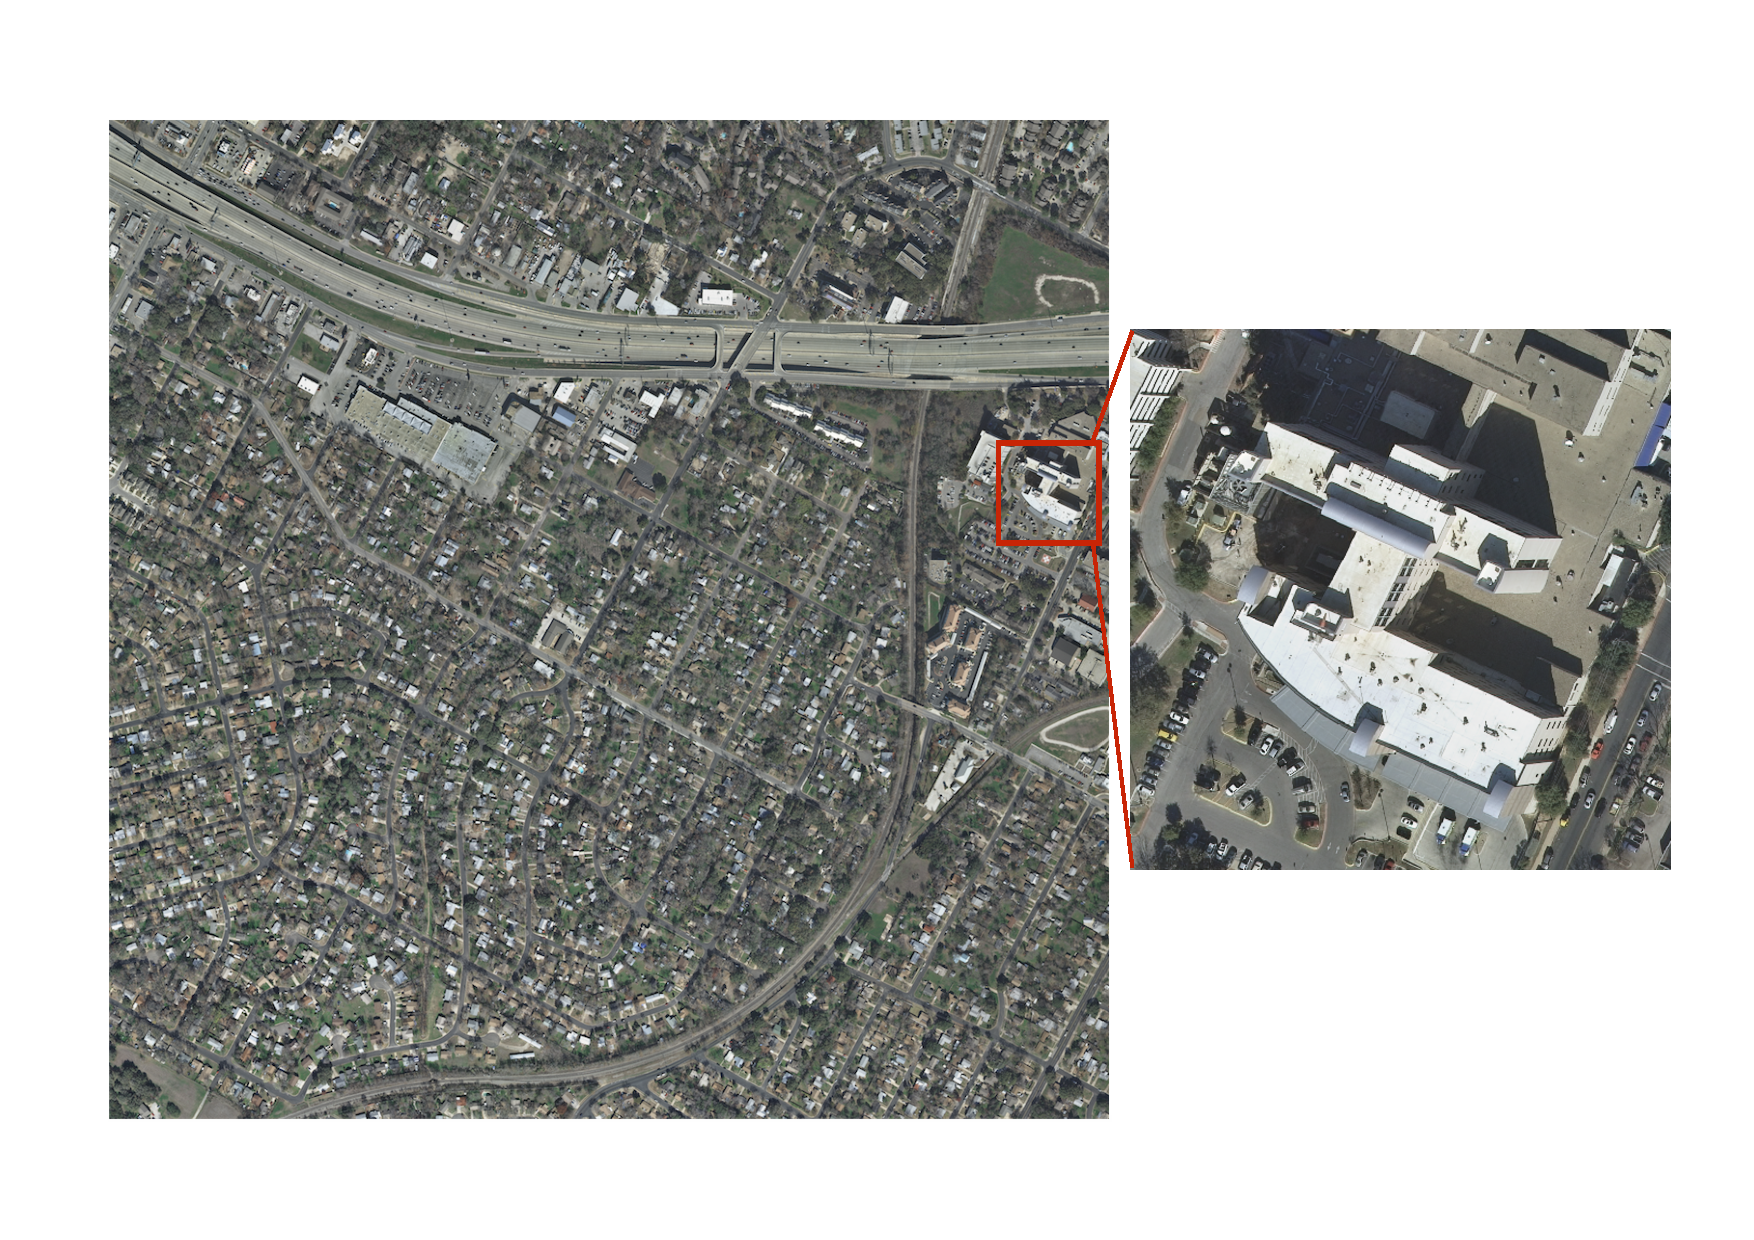
\includegraphics[width=12.0cm]{Austin.pdf}
    \caption{训练集中的一张原始图片。这张图是奥斯丁的照片。}
    \label{fig:Fig 1}
    \end{figure}
    我们先将原先大小为$5000\times5000$的图片补成$5120\times5120$($padding=60$)的大小。然后将按照步长160($stride=160$)其顺序切成961张$320\times320$的小图。\\
    我们随后对图片做的数据增强如下:
    \begin{itemize}
        \item 将图片旋转一个随机的角度
        \item 将图片随机水平/竖直翻转
        \item 加入高斯噪声
        \item 随机调整图片的亮度、对比度、饱和度和色调
    \end{itemize}
    同时也对标签做相同的旋转和翻转的变换。\\
    \begin{figure} [!]
    \centering
    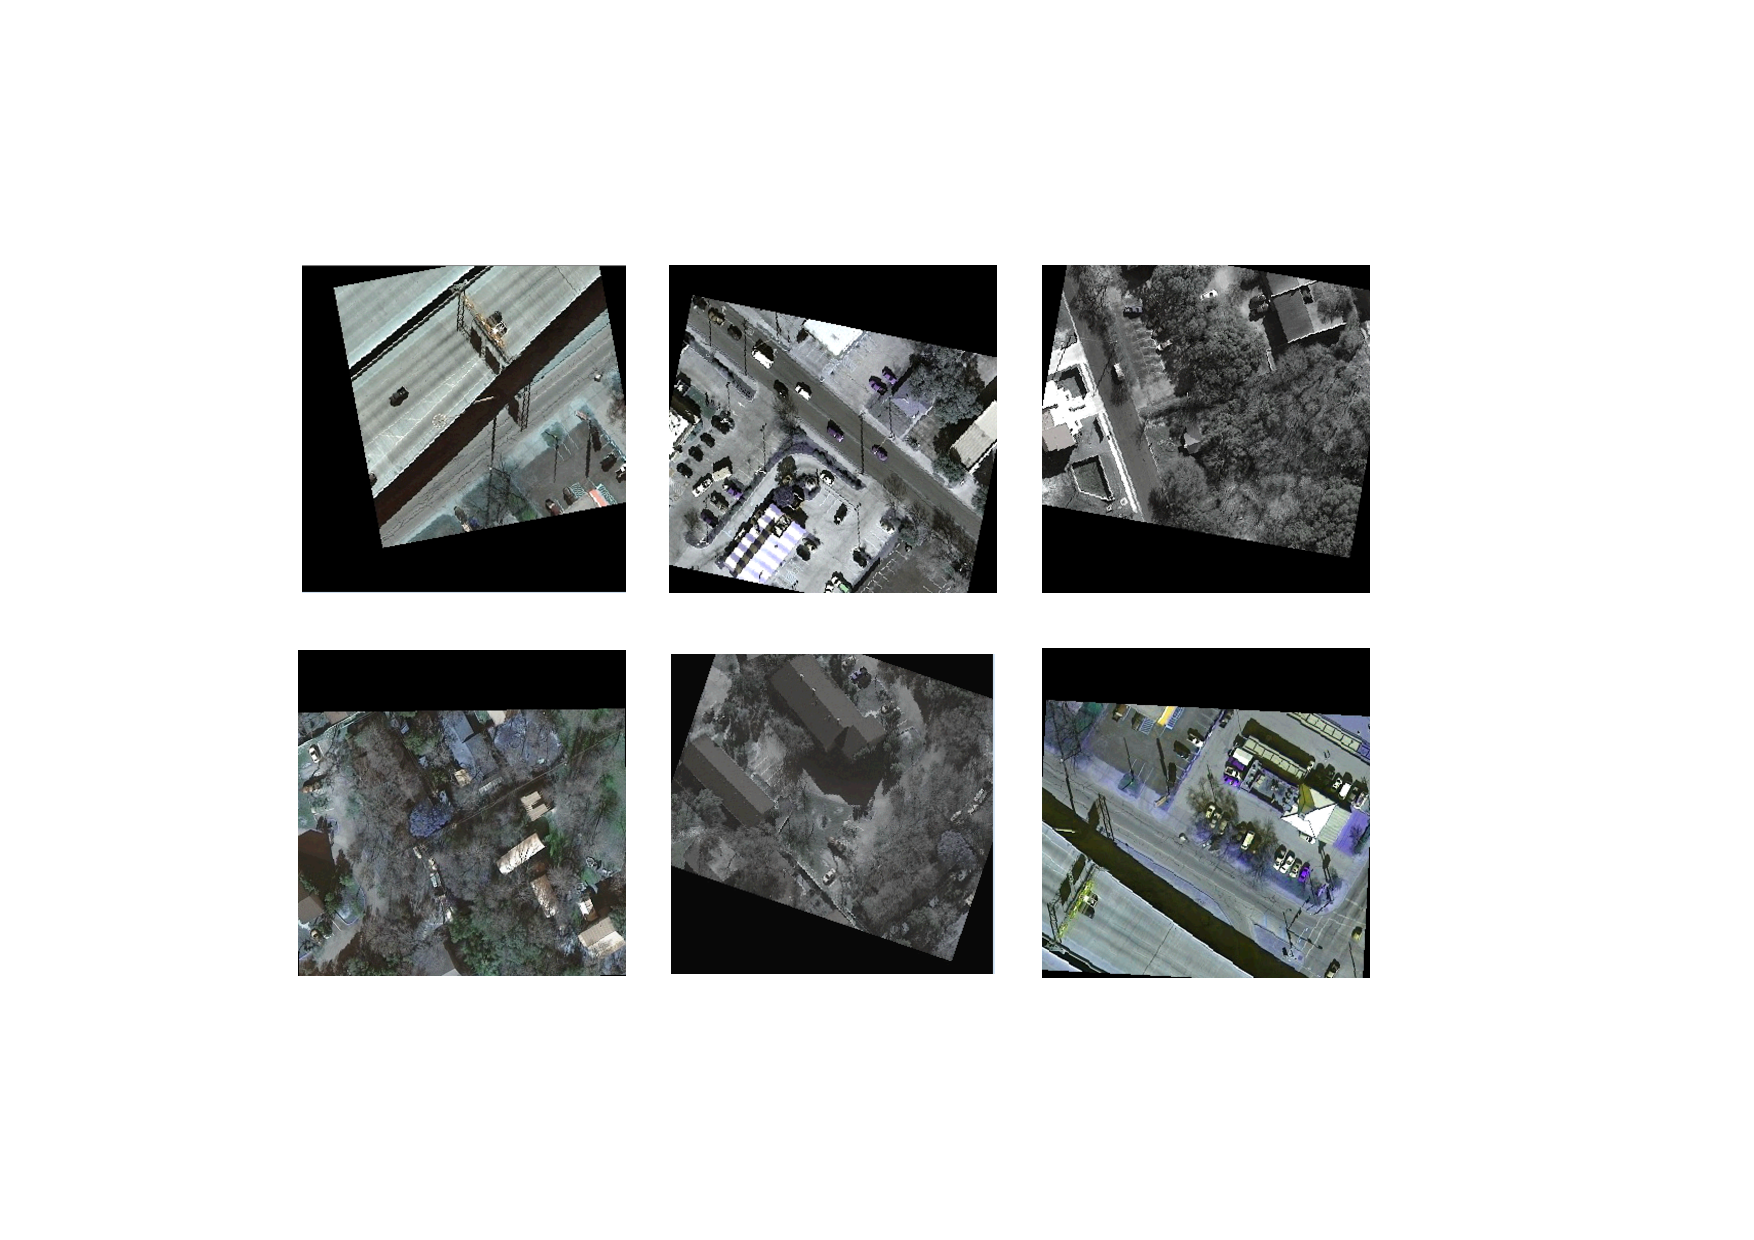
\includegraphics[width=10.0cm]{DataAug.pdf}
    \caption{数据增强的一些例子。旋转会导致图片中黑色边缘的产生。}
    \label{fig:Fig 1}
    \end{figure}
    我们之所以这样进行数据增强,是基于如下几点考虑:
    (1)对于美国城市而言,房子的方向大多是比较统一的,而同一张卫星照片的拍照方向是确定的,将造成训练集中大量的房屋方向相同,这样将使训练数据过于局限。因此,我们决定引入图片的旋转和翻转,这样可以加入随机性,从而增强网络的泛化性能。
    
    (2)由于不同城市的房屋整体色调有所不同,我们希望淡化网络对特定颜色的认知,而主要提取形状特征,这样调整图片的色调就是必要的。
    
    (3)卫星拍照时,所使用的设备不同,可能会导致拍摄图片的信噪比不同。一般而言,拍摄照片时引入的噪声可以用高斯噪声来建模。为了增强网络的鲁棒性,我们还对输入训练数据加入了高斯噪声,噪声的均方差调整为$sigma=0.04$。
    
    与之相对地,我们没有改变图像的尺度。原因在于,在所使用的数据集中,测试集和训练集的图片分辨率均为$0.3$ m,如果在这个数据集上评估,就并不需要改变图像的尺度。然而,这就对我们模型的应用产生了一定的限制——如果用于测试的图片分辨率相差比较大,很可能性能会变差。这一点在之后对北京等城市的评估中有所体现。




    \section{网络结构}
    任务本身属于语义分割。用深度学习进行语义分割的方法多种多样,在本次任务中我们决定采用U-Net,如图所示。
    \begin{figure} [!]
    \centering
    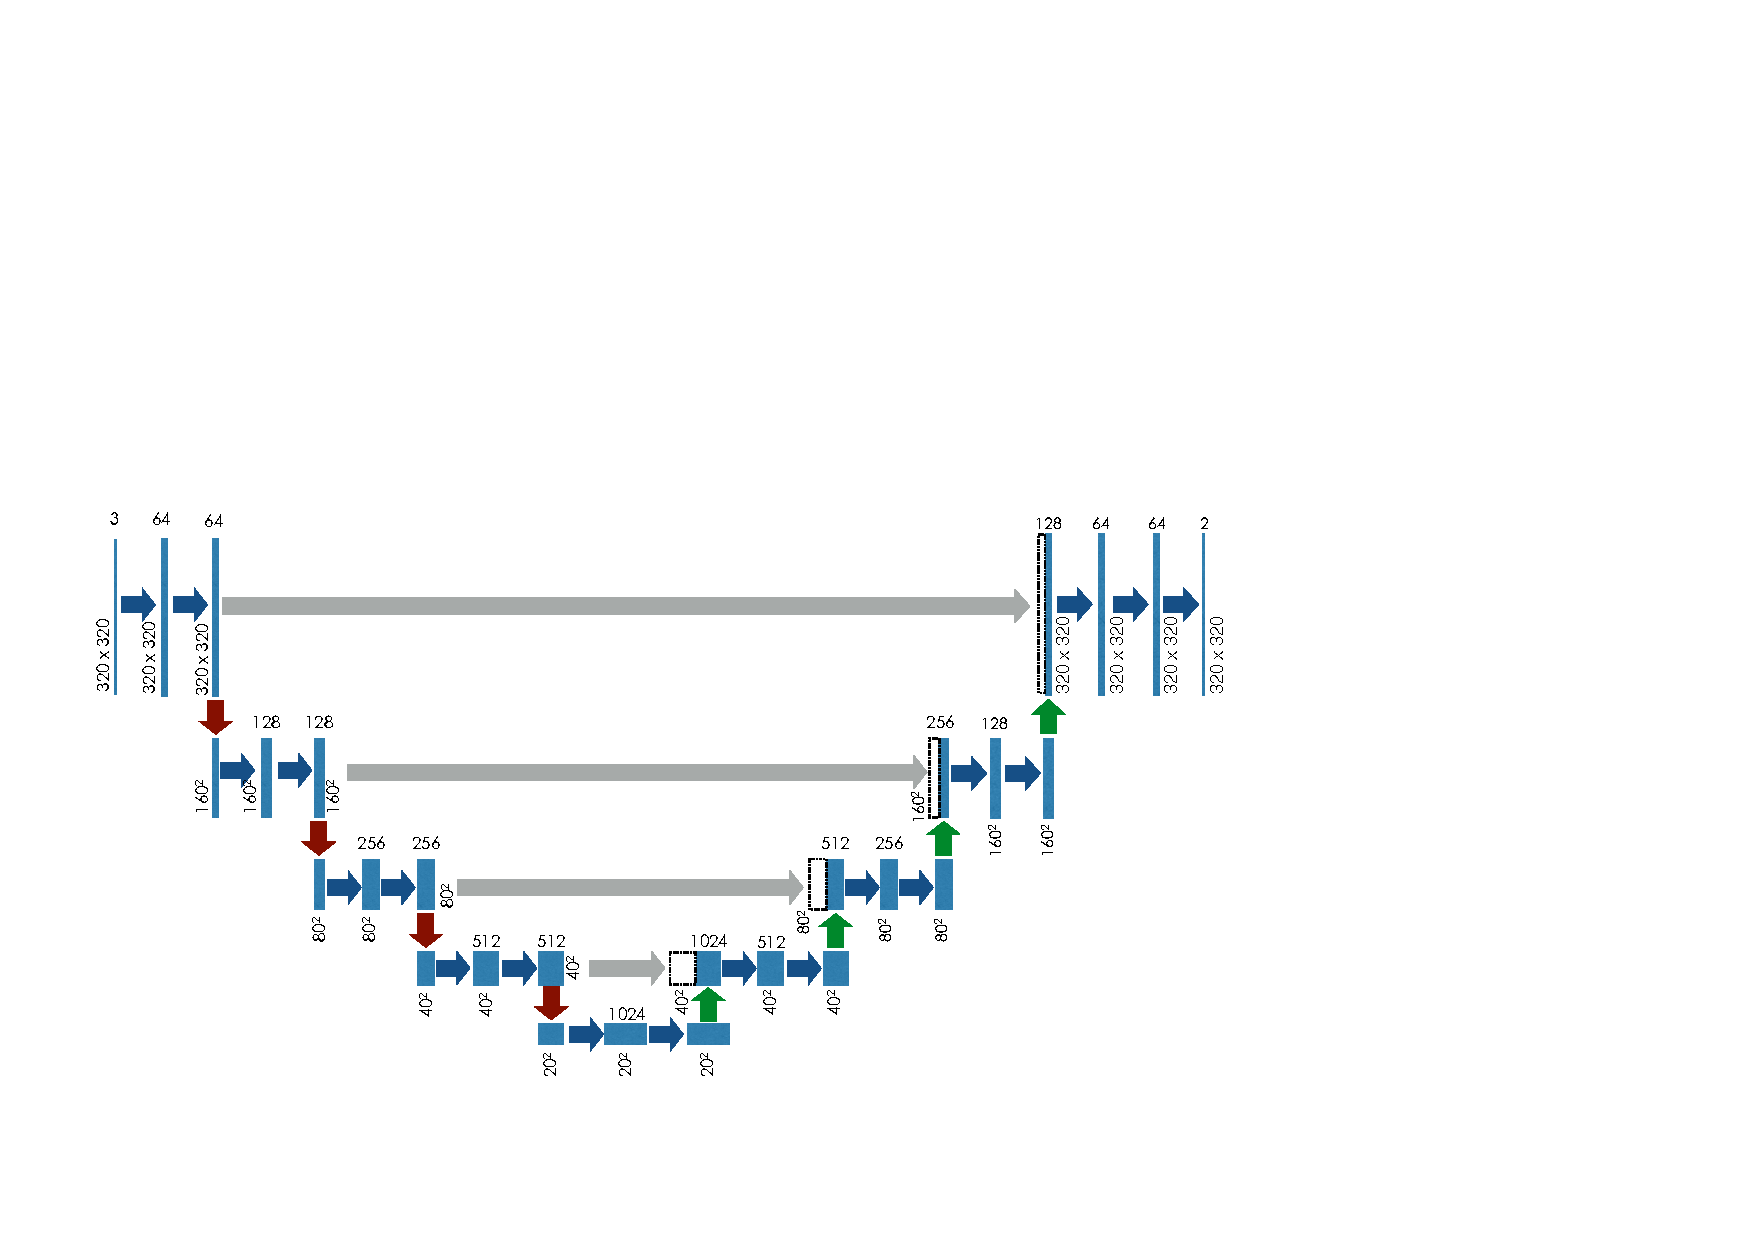
\includegraphics[width=14.0cm]{U_Net.pdf}
    \caption{A schematic illustration of U-Net's structure.}
    \label{fig:Fig 1}
    \end{figure}
    采用U-Net的原因主要是由于结构清晰:属于典型的Encoder-Decoder架构,专门为分割任务设计,考虑到单纯的Encoder-Decoder型网络会丢失图片细节,加入了short-cut,通过将不同尺度的信息进行拼接的方式,缓解了细节的丢失。
    
    最初使用一个U-Net进行测试的效果并不是很理想,于是我们尝试将两个U-Net拼接在一起,希望通过增加模型的深度,取得更好的效果。然而在训练时,拼接的模型很快就出现了过拟合现象,在验证集上的loss无法很好地收敛,泛化性能很差,因此最终我们没有采用这一模型。
    
    \subsection{Loss函数}
    如果简单地把分割任务看作一个二分类,在网络的最后一层使用Softmax激励函数,得到每个像素分属于两类(建筑/非建筑)的概率,那么可以直接用交叉熵作为Loss函数。从代码train.py中可以看到,pyTorch中对于分割问题的Loss,使用的是Nllloss()函数,此时网络最后一层是logsoftmax,但本质是相同的。
    
    对于二分类问题,交叉熵的表达式可以写作:
    \begin{equation}
    L = -\frac{1}{N}\sum[y_{i}\ln(p_{i}) + (1-y_{i})\ln(1-p_{i})].
    \end{equation}
    在模型V1.0中,我们直接使用交叉熵作为Loss函数,效果比较差,存在很多大量False negative,很多建筑物无法判断出来。False negative较多的主要原因是正负样本不均衡,因此在此后的模型中,我们决定调整交叉熵表达式中两项的权重。根据参考文献\cite{},最直接的解决方法是计算正负两类所占的比例$\alpha_{0}$和$\alpha_{1}$(自然满足$\alpha_{0}+\alpha_{1}=1$),然后将两项分别乘上对应的系数:
    \begin{equation}
    L = -\frac{1}{N}\sum[\alpha_{0}y_{i}\ln(p_{i}) + \alpha_{1} (1-y_{i})\ln(1-p_{i})].
    \end{equation}
    经过统计,在数据集中,建筑物对应的像素所占比例约为$15\%-20\%$,因此在模型V1.2中,采用比例$\alpha_{1}=0.2$。这样,如果对于某个像素满足$y_{i}=1$,但预测${p_{i}}$明显小于1,乘以$\alpha_{0}$相当于对此类情形施加惩罚,从而一定程度上解决正负样本不均的问题。
    
    一般而言,针对语义分割任务,一个重要的评价标准是IoU。实际上IoU比单纯计算准确率更加合理(对于建筑物只占$15\%$的情形,预测全0便可以达到$85\%$的准确率)。对于一个类别而言,记预测的mask为$X$,实际的mask为$Y$,IoU的定义为:
    \begin{equation}
    \rm{IoU} = \frac{\left |{X}\bigcap{Y}\right |}{\left |{X}\bigcup{Y}\right |}.
    \end{equation}
    
    经过查阅资料\cite{},针对IoU可以设计更为合理的Loss。根据$Y$和预测的$X$定义Dice系数:
    \begin{equation}
    \rm{DSC} = \frac{2 \left |{X}\bigcap{Y}\right |}{\left |X \right |+ \left |Y\right |}.
    \end{equation}
    直观来说,Dice系数形式上比较接近IoU。为了达到最大化IoU的目的,可以尝试将Dice系数加入Loss函数。包含$X$的Dice系数是不可导的,因此记$P$为预测的概率(不转化为0/1标签),定义非负的$\rm{DSC}_{diff}$为:
    \begin{equation}
    \rm{{DSC}_{diff}} = \frac{2\sum y_{i}p_{i}}{\sum p_{i} + \sum{y_{i}}}.
    \end{equation}
    当完美预测时(所有标签为1的像素,预测为建筑的概率均为$1$),$\rm{DSC}_{diff}$达到1。在Kaggle比赛中,有人采用$1-\rm{DSC}_{diff}$作为Loss函数中的一项。在本次实验中,为了对IoU较小的预测施加更大的惩罚力度,我们将$-\ln(\rm{DSC}_{diff})$加入Loss函数中(在$\rm{DSC}_{diff}$接近1的时候二者相近)。对于模型V1.4,我们采用如下形式的Loss函数进行训练:
    \begin{equation}
    L = -\frac{1}{N}\sum[(1-\alpha_{1})y_{i}\ln(p_{i}) + \alpha_{1} (1-y_{i})\ln(1-p_{i})] - \beta \ln(\rm{DSC}_{diff}).
    \end{equation}
    
    我们在报告后面会对各个不同模型进行测试,测试条件和结果汇总在表格当中。

    \section{条件随机场(CRF)}
    条件随机场(Conditional Random Field)是一种判别式概率模型,具有无向的图模型\cite{}。实际上,对于图像分割的任务而言,CRF属于传统算法。在谷歌的DeepLab中\cite{},CRF被用于与深度神经网络结合,作为后处理的手段。迄今为止,DeepLab在诸多图像分割数据集(VOC, Cityscapes)上都达到了相当不错的效果,展现了深度学习方法与CRF结合的潜力。

    在DeepLab的论文中,神经网络的输出被作为先验概率,如果直接使用这一概率进行分割,结果是很粗糙的(特别是在两类的边缘附近),即便加入short-cut也无法完全解决细节丢失的问题。CRF则根据神经网络的输出,借助像素的位置和颜色信息,计算后验概率。在区域中间部分,先验概率远离阈值,基本不会受到CRF的影响;在两区域边缘处,CRF进行后处理的主要依据则是像素颜色,处理之后可以达到比较精细的分割结果。

    参考论文\cite{},采用全连接CRF进行图像分割,吉布斯自由能为:
    \begin{equation}
    E(\textbf{x}) = \sum_{i} \phi_{u}(x_{i}) + \sum_{i, j} \phi_{p} (x_{i}, x_{j}).
    \end{equation}
    第二项为成对的像素对应的能量,表达式为:
    \begin{equation}
    \phi_{p}(x_{i}, x_{j}) = \mu(x_{i}, x_{j}) k(\textbf{f}_{i}, \textbf{f}_{j}),
    \end{equation}
    其中,核$k(\textbf{f}_{i}, \textbf{f}_{j})$的表达式采用如下形式:
    \begin{equation}
    k(\textbf{f}_{i}, \textbf{f}_{j}) = w^{(1)}\exp[-\frac{\| p_{i} - p_{j}\| ^{2}}{2\theta_{\alpha}^{2}} - \frac{\| I_{i} - I_{j}\| ^{2}}{2\theta_{\beta}^{2}}] + w^{(2)} \exp[-\frac{\| p_{i} - p_{j}\| ^{2}}{2\theta_{\gamma}^{2}}].
    \end{equation}

    在CRF算法中,涉及到诸多参数。在本次实验当中,用CRF进行后处理并不是任务最主要的部分,只是作为一种尝试。因此我们采用了一个轻量级的名为pydensecrf的库(github网址),然后人为设定了相应的参数,并根据部分图片的处理情况进行了一定的调整。

    \begin{figure} [!]
    \centering
    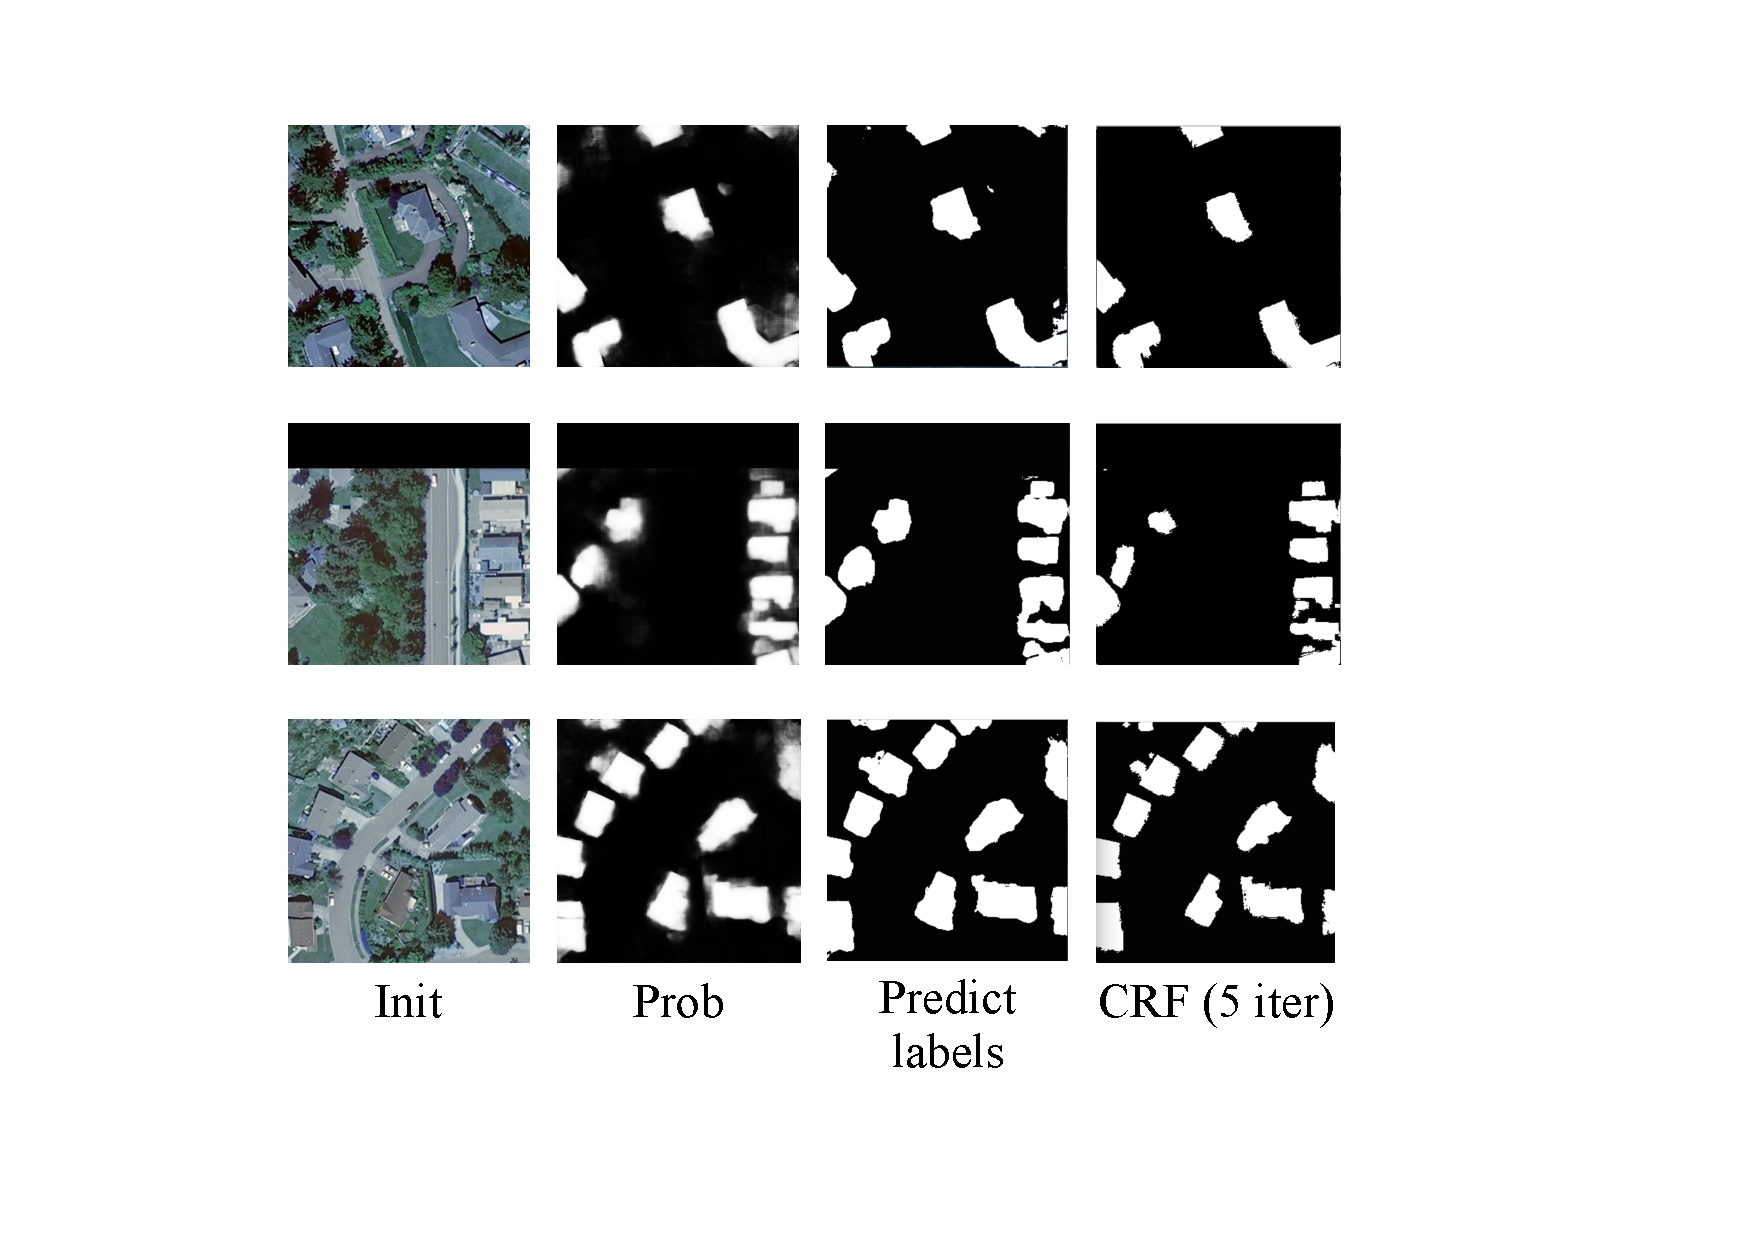
\includegraphics[width=14.0cm]{CRF_1.pdf}
    \caption{借助CRF进行后处理的一些例子。不难看到,几次迭代之后,预测mask的边缘变得比较锐利,小块的false positive被消除,IoU得到了改善。}
    \label{fig:Fig 2}
    \end{figure}

    经过尝试,我们发现,尽管人为调整CRF的参数$\theta_{\alpha}$、$\theta_{\beta}$、$\theta_{\gamma}$可以在一个小区域内达到比较好的结果,但是这一组参数用于其他区域的效果可能不尽人意(泛化性能较差)。这一现象并不难理解:首先,不同城市的建筑/非建筑色调差异很大;其次,即便是同一城市,若照片的拍摄时间、地点不同,也会存在较明显的光照差异,影响到像素点的颜色。本次实验采取的CRF算法比较简单,只考虑到一对像素点之间的能量,特征选取也很简单,仅包括位置和颜色,本身鲁棒性不够强。

    对于我们的模型而言,CRF比较重大的意义在于,通过后处理,可以将小块的false positive去掉,改善分割结果。
    \begin{figure} [!]
    \centering
    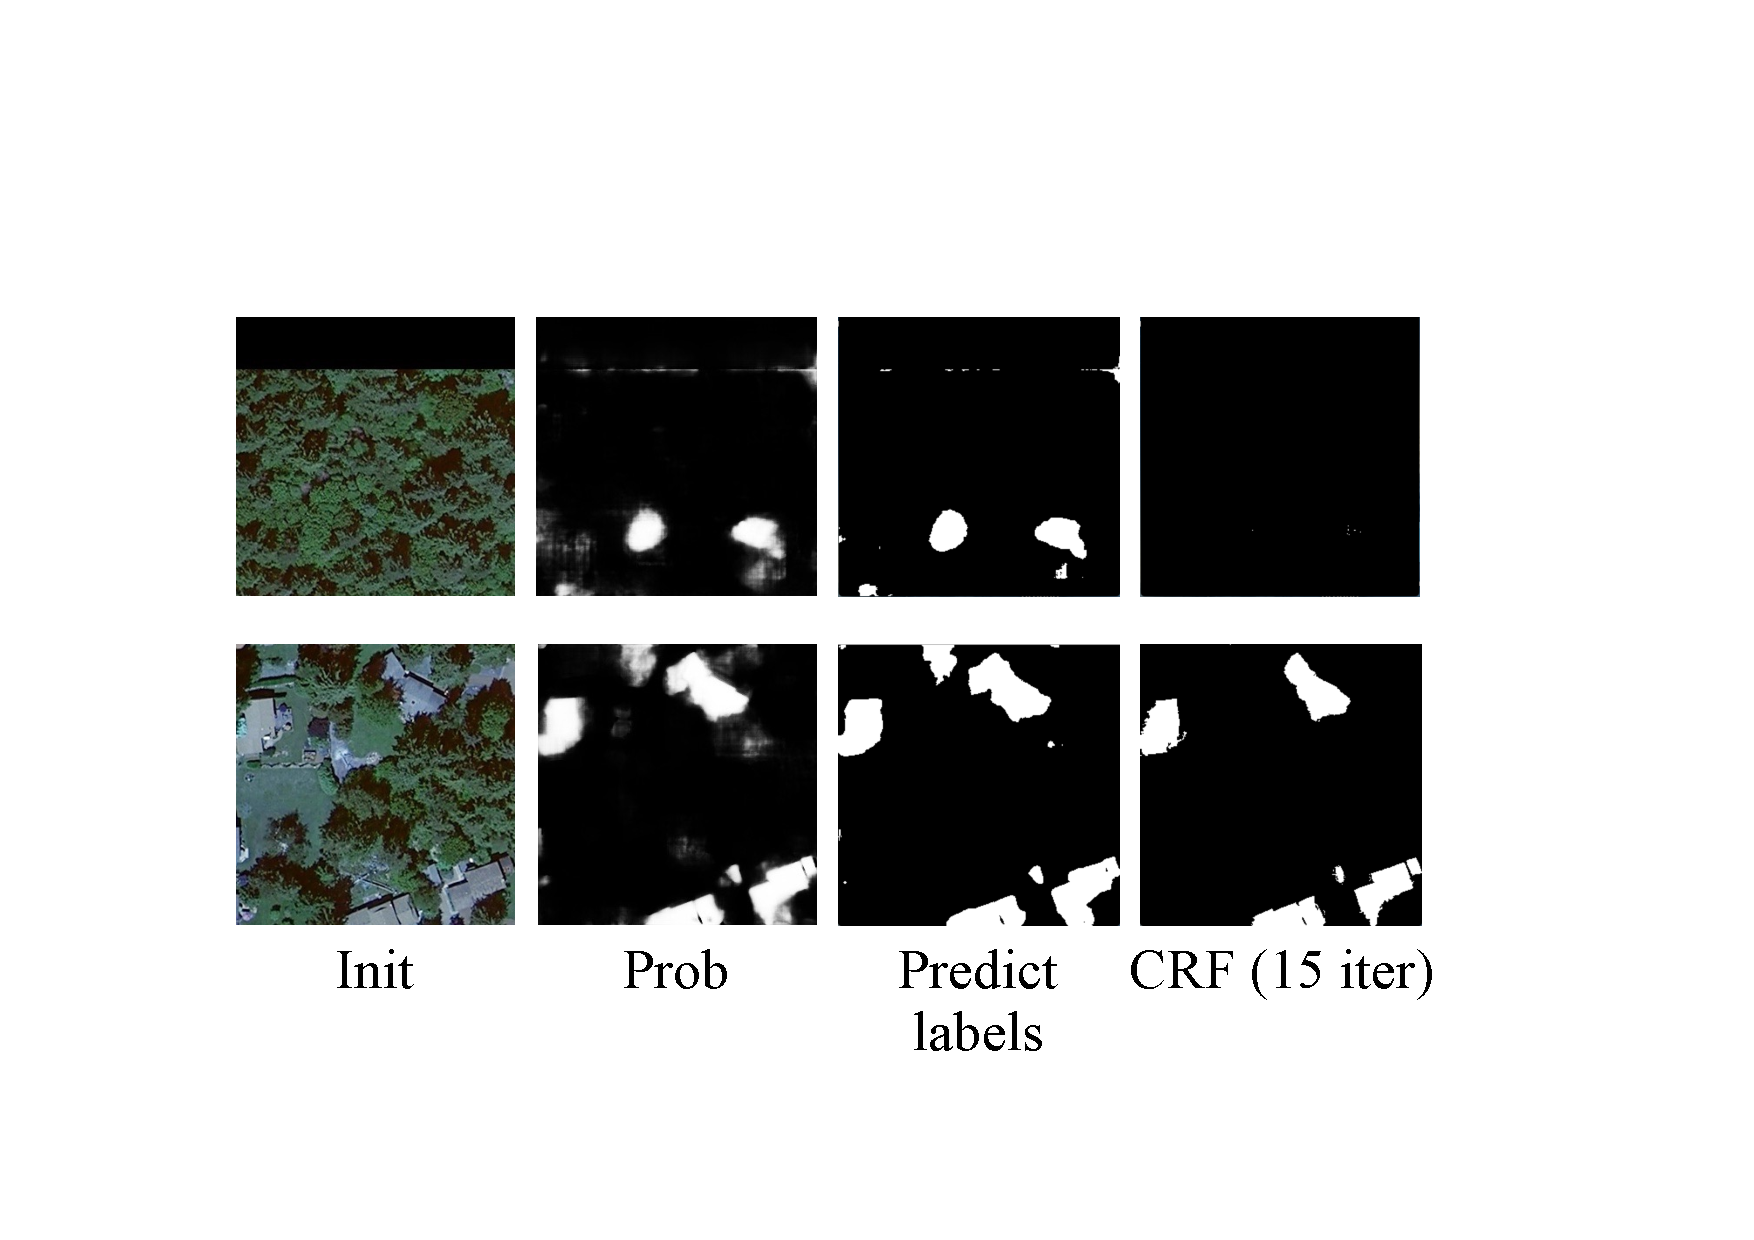
\includegraphics[width=14.0cm]{CRF_2.pdf}
    \caption{CRF可以去除掉false positive,改善分割结果。}
    \label{fig:Fig 2}
    \end{figure}
    然而,如果参数设置不合理,可能会出现将true positive的一部分去除的情况(例如,由于屋顶有角度,向光与背光两面的颜色差异比较大,CRF后处理之后只保留了向光的部分)。因此,在使用条件随机场进行后处理时必须谨慎。
    \begin{figure} [!]
    \centering
    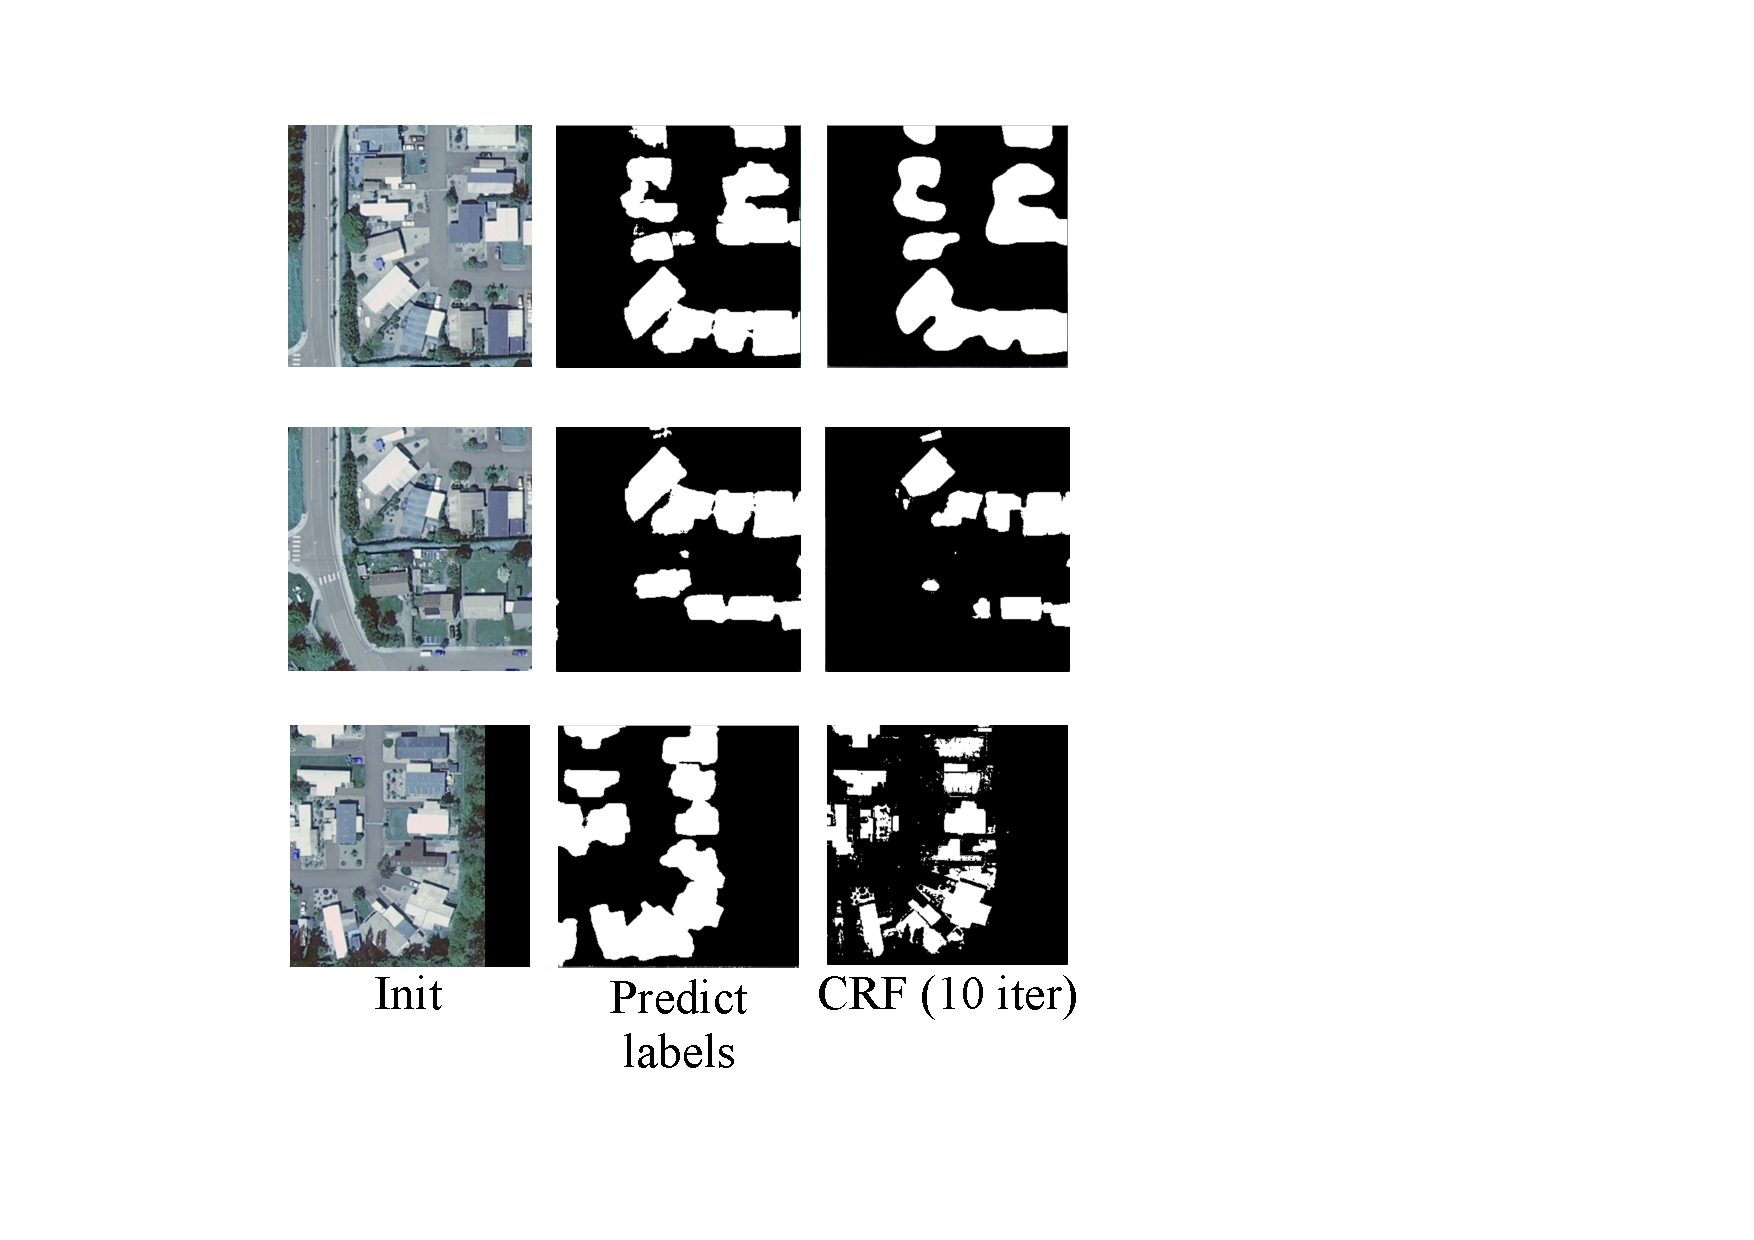
\includegraphics[width=10.0cm]{CRF_3.pdf}
    \caption{如果参数设置不合理,可能导致后处理之后效果反而变差,几种典型的情况如图。}
    \label{fig:Fig 3}
    \end{figure}



    
    \section{模型评估}
    对于INRIA的数据集,训练集和测试集分别包含180张大图。测试集的标签是无法拿到的,如果想知道准确率,唯一的手段是将预测的mask打包上传,由INRIA的工作人员进行评价。然而,我们试图将结果提交到网站上时,遇到了难以解决的技术问题,向工作人员发送邮件也没有得到回复。因此,我们最终评价模型时,只能通过验证集IoU和典型例子来进行评价。
    \subsection{评估方式}
    在进行Inference时,仍然将测试集的所有图片(大小$5000\times5000$)补为$5120\times5120$,并划分为$320\times320$,stride为$160$。将每个$320\times320$的图片进行inference,计算概率,并在整张大图上进行平均,以概率阈值$0.5$进行二分类,最后再取中央的$5000\times5000$,从而得到完整的mask。
    
    原始数据的训练集包含来自5个城市的180张图片。在每个城市的36张图片中,我们将前31张用于训练,后5张用于验证。我们计算了各个模型在验证集上的准确度和IoU,进行比较。
    \subsection{模型汇总}
    我们训练了许多模型,在报告中只针对比较有代表性的4个进行评估。各个版本模型的异同汇总在下列表格当中。
    \begin{table}[!]
    \caption{Typical Parameter Values.}
    \label{tab:parameters}
    \centering
    \begin{tabular}{ccc}
	\hline
	\hline
	Version & Loss & Net \\
	\hline
	1.0 & Cross Entropy & U-Net \\
	1.1 & Weighted Cross Entropy & U-Net \\
	1.2 & Weighted Cross Entropy & 2$\times$U-Net \\
	1.3 & Weighted Cross Entropy + DICE & U-Net \\
	\hline
	\hline
    \end{tabular}
    \end{table}
    这四个模型在验证集上的准确率(Acc)和IoU分别如下表所示:
    \begin{table}[!]
    \caption{Typical Parameter Values.}
    \label{tab:parameters}
    \centering
    \begin{tabular}{ccc}
	\hline
	\hline
	Version & Val Acc/$\%$ & Val IoU \\
	\hline
	1.0 & &  \\
	1.1 & &  \\
	1.2 & &  \\
	1.3 & &  \\
	\hline
	\hline
    \end{tabular}
    \end{table}
    \subsection{评估~\& 测试例子}
    在测试集图片上对4个模型分别进行简单测试。由于我们无法获得测试集的标签,只能根据少数测试样例的分割情况进行简单判断,再结合经验进行分析。
    
    (1)V1.0:由于简单使用没有加权的交叉熵作为Loss函数,在正负样本严重不均的情况下,会出现相当多的false negative,对于密集的建筑物几乎无法识别。
    \begin{figure} [!]
    \centering
    \includegraphics[width=10.0cm]{V0.png}
    \caption{模型V1.0无法完成分割任务,这是由于训练集中正负样本不均。}
    \label{fig:Fig 3}
    \end{figure}
    
    (2)V1.1:为了解决正负样本不均的问题,采用加权的交叉熵,系数$\alpha_{1}=0.2$。训练集不变。
    \begin{figure} [!]
    \centering
    \includegraphics[width=10.0cm]{V1.png}
    \caption{模型V1.1可以初步完成分割任务,但效果还比较差。}
    \label{fig:Fig 3}
    \end{figure}
    虽然已经具备一定的效果,但遗漏情况仍然存在,并且存在把人行道误判为建筑的情况。
    
    (3)V1.2:尝试将两个U-Net简单堆叠,希望取得更好的效果。
    \begin{figure} [!]
    \centering
    \includegraphics[width=10.0cm]{V2.png}
    \caption{测试时发现,模型V1.2的总体表现不如V1.1,这是因为深度网络容易过拟合。}
    \label{fig:Fig 3}
    \end{figure}

    训练过程中,训练集的Loss下降很明显,但验证集的Loss波动十分剧烈,并且很快就开始上升,说明网络过拟合。由于无法进一步充实数据集,我们决定回归到单个U-Net。
    
    (4)V1.3:使用单个U-Net,改变Loss——除加权交叉熵外,引入DICE系数,直接目的是提升IoU。
    \begin{figure} [!]
    \centering
    \includegraphics[width=5.0cm]{V3.png}
    \caption{模型V1.3的分割效果比较令人满意,但仍然存在少许误判。}
    \label{fig:Fig 3}
    \end{figure}
    
    虽然仍然存在少许误判,但绝大部分房屋都没有遗漏,从效果上看,边缘处的分割也做的不错。在之后的部分,我们将重点观察分析模型V1.3的优缺点,并提出一些可能的改进方向。
    



    \section{在中国的应用效果}
    不忘初心,继续前进。之前所做的工作和训练的模型,都是为了实现我们进行中国地区的土地利用情况而服务的。为了测试其效果,我们从谷歌地图上\cite{}截取了北京城市地区和农村地区、上海城市地区和江苏农村地区的部分遥感卫星地图放进网络进行试验,效果如下:
    \begin{figure}
        \centering
        \subfigure[原图]{
        \label{figa} %% label for first subfigure
        \includegraphics[scale=.4]{BJ_construct.png}}
        \hspace{1in}
        \subfigure[小框]{
        \label{figa} %% label for first subfigure
        \includegraphics[scale=.4]{BJ_rural_house.png}}
        \hspace{1in}
        \subfigure[中框]{
        \label{fig:subfig:b} %% label for second subfigure
        \includegraphics[scale=.4]{BJ_rural_field.png}}
        \hspace{1in}
        \subfigure[大框]{
        \label{figb} %% label for first subfigure
        \includegraphics[scale=.4]{SH_downtown.png}}
        \hspace{1in}
        \subfigure[大框]{
        \label{figb} %% label for first subfigure
        \includegraphics[scale=.4]{JS_rural.png}}
        \caption{我们发现,当框图最小时,切出来的grabcut结果最符合直觉上的美感,当框图扩大时,切割结果  就会或多或少出现问题,这是因为当我们从很小开始时,范围不断扩大这个过程的鲁棒性比从大框往里面缩的  效果要好,因此我认为,这种情况小比大更合适}
        \label{figb} %% label for entire figure
    \end{figure}

    
    \bibliography{reference}
    
\end{spacing}
\end{CJK*}
\end{document}